\documentclass[12pt,a4paper,twocolumn]{article}
\usepackage{bachelorproject}
\usepackage{pgfplots}
\pgfplotsset{compat=1.12}
\usepackage{lmodern}
\usepackage{footmisc}
\usepackage{amsmath}
\usepackage{amssymb}
\usepackage{mathabx}
\usepackage{amsthm}
\usepackage{mathtools}


\usetikzlibrary{shapes,snakes}

\newcommand{\KP}[1]{%
	\begin{tikzpicture}[baseline=-\dimexpr\fontdimen22\textfont2\relax]
		#1
	\end{tikzpicture}%
}
\newcommand{\KPA}{%
	\KP{\filldraw[color=gray, fill=none, thick] circle (0.3);}%
}
\newcommand{\KPB}{%
	\KP{
		\draw[color=gray,thick] (-0.3,-0.3) -- (0.3,0.3);
		\draw[color=gray,thick] (-0.3,0.3) -- (-0.05,0.05);
		\draw[color=gray,thick] (0.05,-0.05) -- (0.3,-0.3);
	}%
}
\newcommand{\KPC}{%
	\KP{%
		\draw[color=gray,thick] (-0.3,-0.3) .. controls (0.05,0) .. (-0.3,0.3);
		\draw[color=gray,thick] (0.3,-0.3) .. controls (-0.05,0) .. (0.3,0.3);
	}%
}
\newcommand{\KPD}{%
	\KP{%
		\draw[color=gray,thick] (-0.3,0.3) .. controls (0,-0.05) .. (0.3,0.3);
		\draw[color=gray,thick] (-0.3,-0.3) .. controls (0,0.05) .. (0.3,-0.3);
	}%
}
\newcommand{\KPI}{%
	\KP{
		\draw[color=gray,thick] (-0.3,0.3) -- (0.3,-0.3);
		\draw[color=gray,thick] (-0.3,-0.3) -- (-0.05,-0.05);
		\draw[color=gray,thick] (0.05,0.05) -- (0.3,0.3);
	}%
}


\title{Nusos i el polinomi de Jones}
\author{Guillem Tutusaus Alcaraz, 1533701, 1533701@uab.cat}
%\text{Universitat Autònoma de Barcelona, Cerdanyola del Vallès}
\supervisors{Joan Porti Piqué}
\begin{document}
	\twocolumn[
	\maketitle
	\begin{@twocolumnfalse}
		\begin{abstract}
	Aquest és un document que tracta de donar una primera introducció a la teoria de nusos, estudiar alguns dels seus invariants algebràics més coneguts posant una ènfasis especial en el polinomi de Jones i classificar d'aquesta manera els nusos d'ordre més baix. Finalment, en buscarem algunes aplicacions.
	\vspace{6ex}
\end{abstract}

		%\tableofcontents
	\end{@twocolumnfalse}
	]
	
	\thispagestyle{firststyle}
	
	% !TEX root = thesis.tex
\renewcommand{\figurename}{Figura}
\renewcommand{\proofname}{Demostració}
\newtheorem{definition}{Definició}
\newtheorem{theorem}{Teorema}
\newtheorem{proposition}{Proposició}
\newtheorem{corolary}{Corol·lari}
\newtheorem{lemma}{Lema}

\section{Introducció}\label{sec:Introducció}
L'espècie humana té coneixement dels nusos desde temps prehistòrics. Començant per l'enregistrament d'informació, les xarxes de pesca i fins i tot per motius religiosos, els nusos han estat de gran importància per la seva utilitat i simbologia espiritual. Moltes obres d'art de cultures d'arreu del món presenten aquestes figures en les seves obres. Alguns exemples son la cultura Xinesa, Tibetana o Celta.\\

Els nusos comencen a tenir la seva presència dins el món de les matemàtiques a partir de l'any 1771 degut als treballs realitzats per Alexandre-Théophile Vandermonde el qual es dedicà a estudiar les propietats topològiques dels nusos en relació a la seva posició en l'espai. Treballs posteriors de Carl Friedrich Gau\ss$ $ qui va definir diverses propietats d'aquests objectes [\cite{knottheory}] van projectar aquesta teoria a la fama. L'any 1860 la teoria sobre l'atom en l'aether formulada per William Thomson va dur a Peter Guthrie Tait a la creació de les primeres taules de nusos. L'any 1885, aquest va publicar la primera taula amb tots els nusos de fins a deu creuaments, també va formular les conjectures que duen el seu nom.\\

A principis del segle XX, Max Dehn i J. W. Alexander van estudiar els nusos des del punt de vista de la teoria de grups i el seus invariants utilitzant grups d'homologia, cosa que va dur a la creació d'un dels primers invariants algebràics de la teoria, el polinomi d'Alexander.\\

A finals de l'any 1970, la incorporació de la geometria hiperbòlica en l'estudi dels nusos utilitzant el teorema de Geometrització de Thurston va permetre classificar aquests en funció de la seva mètrica, permetent l'ús de la geometria en la creació de nous invariants. El descobriment del polinomi de Jones per part de Vaughan Jones l'any 1984 [\cite{mathwithatwist}] juntament amb contribucions de Edward Witten i Maxim Kontsevich van revelar fortes relacions entre la teoria de nusos i mètodes matemàtics en mecànica estadística i teoria quàntica de camps. Una gran quantitat de invariant han estat inventats desde llavors utilitzant eines com els grups quàntics o la homologia de Floer.\\

En les darreres dècades, els científics han estat interessats en l'estudi dels nusos físics per tal de comprendre el nuament de l'ADN i de diferents polímers. Aquesta teoria s'utilitza també per determinar si una molècula és o no quiral. Finalment, la teoria de nusos pot ser crucial en la construcció dels primers ordinadors quàntics a través del model proposat per Alexei Kitaev [\cite{computingwithquantumknots}].\\

\subsection{Sobre els nusos}\label{subsec:sobreelsnusos}
Els nusos, son estructures presents en el nostre dia a dia. Podriem considerar un nus, en el sentit habitual, qualsevol de les figures següents.

\begin{figure}[h]
  \centering
  \includegraphics[width=0.401\linewidth]{img/nus simple.jpg}
  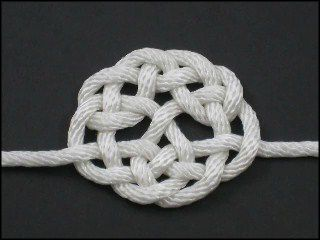
\includegraphics[width=0.535\linewidth]{img/Nus de Dara.jpg}
  \caption{D'esquerra a dreta: Nus simple (Overhand Knot en anglès) i Nus de Dara, nus celta símbol de la força.
  }\label{fig:exemples de nusos}
\end{figure}

El problema que tenen aquests nusos és que, aquests mantenen la seva forma a partir de la tensió i fricció que existeix entre les cordes que formen el nus. No és gaire difícil veure que un podria desfer aquests nusos de manera que acabariem obtenint una simple corda sense cap nus. És per això, que en matemàtiques és necessari considerar una definició més restrictiva d'aquest concepte per tal de preservar-ne l'estructura interna. Podriem pensar, que si uníssim els caps de les cordes de la Figura \ref{fig:exemples de nusos}, aleshores només tallant la corda seriem capaços de desfer el nus (això precisa de demostració!).
	% !TEX root = thesis.tex

\section{Algunes definicions i els objectius de la teoria de nusos}\label{sec:Algunes definicions i els objectius de la teoria de nusos}

De definicions de nus, parlant en termes matemàtics, n'hi ha diverses. Nosaltres considerarem la definició dins el camp de la topologia, d'on en reutilitzarem molta notació. A més, la teoria de nusos s'emmarca dins una teoria més general; la de links. Per tant, moltes vegades anirem mencionant resultats que també son vàlids per aquests objectes. La següent secció pretén donar unes primeres definicions pel que fa als nostres objectes d'estudi.

\begin{definition}\label{def: Definició de nus}
	Diem que $L$ és un \underline{link} de m components, o un m-link si és un subconjunt de $S^3$, o de $\mathbb{R}^3$, que consisteix en m corbes disjuntes, simples, tancades i lineals a trossos. Un 1-link és un \underline{nus}.
\end{definition}

La condició de lineal a trossos significa que les components de $L$ estan cadascuna d'elles feta d'un nombre finit de rectes col·locades una al costat de l'altra amb el principi d'una coincidint amb el final de l'altra. Aquesta condició evita la creació de nusos patològics que no presenten un comportament esperat. A aquests últims nusos se'ls anomena \textit{salvatges} i no seran estudiats en aquest treball. A la pràctica, quan representem nusos o links assumirem que hi ha tants segments rectes que cada component semblarà corba.\\

\begin{figure}
	\centering
	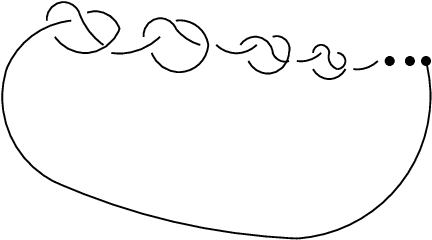
\includegraphics[width=0.9\linewidth]{img/wildknot.png}
	\caption{Exemple d'un nus salvatge.}\label{fig:nussalvatge}
\end{figure}

\textit{De què tracta la teoria de nusos?}
Una possible resposta és que la teoria de nusos pretén classificar el conjunt de possibles nusos. Donat un nus $K$, hom considera que aquest està inclòs, mitjançant una aplicació contínua, dins l'espai ambient tres dimensional $\mathbb{R}^3$ o equivalentment dins $S^3$, obtenim aleshores la teoria clàssica de nusos. Aquesta teoria pretén estudiar la col·locació de $K$ dins aquest espai. Classificar, en aquest cas vol dir considerar iguals sota certes condicions, que definirem més endavant.

\begin{figure}
	\centering
	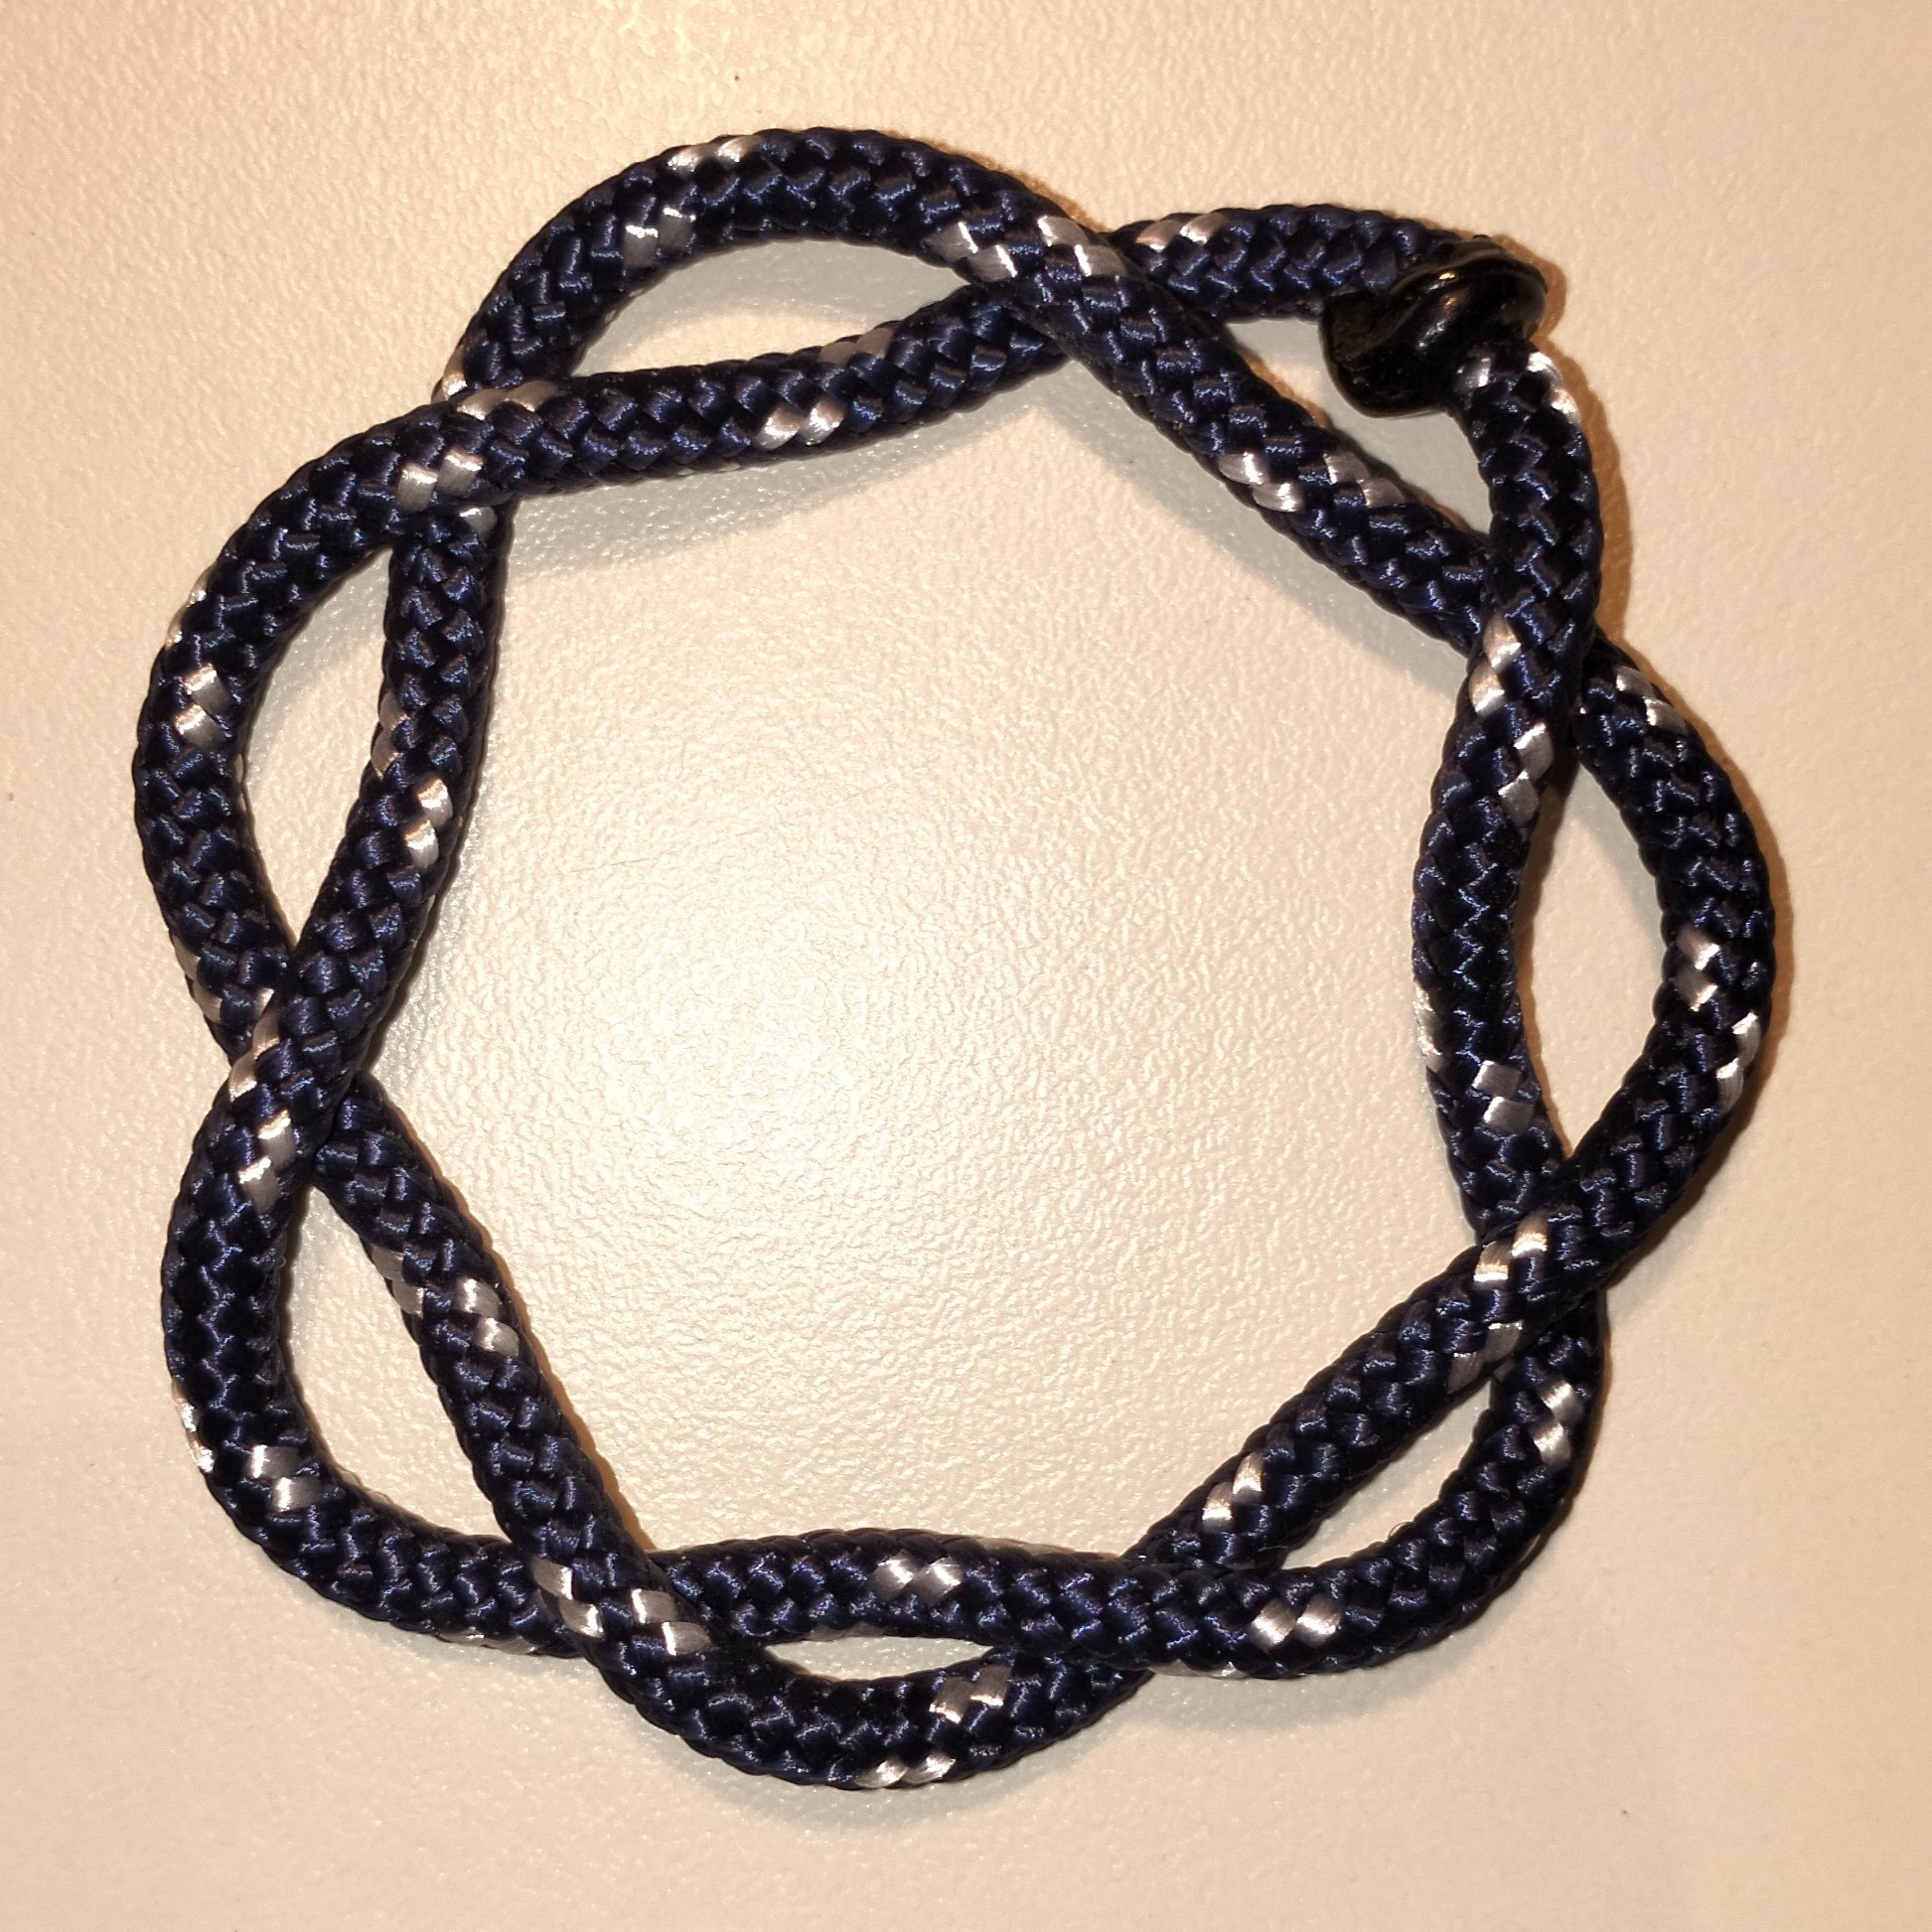
\includegraphics[width=0.45\linewidth]{img/7_1.jpg}
	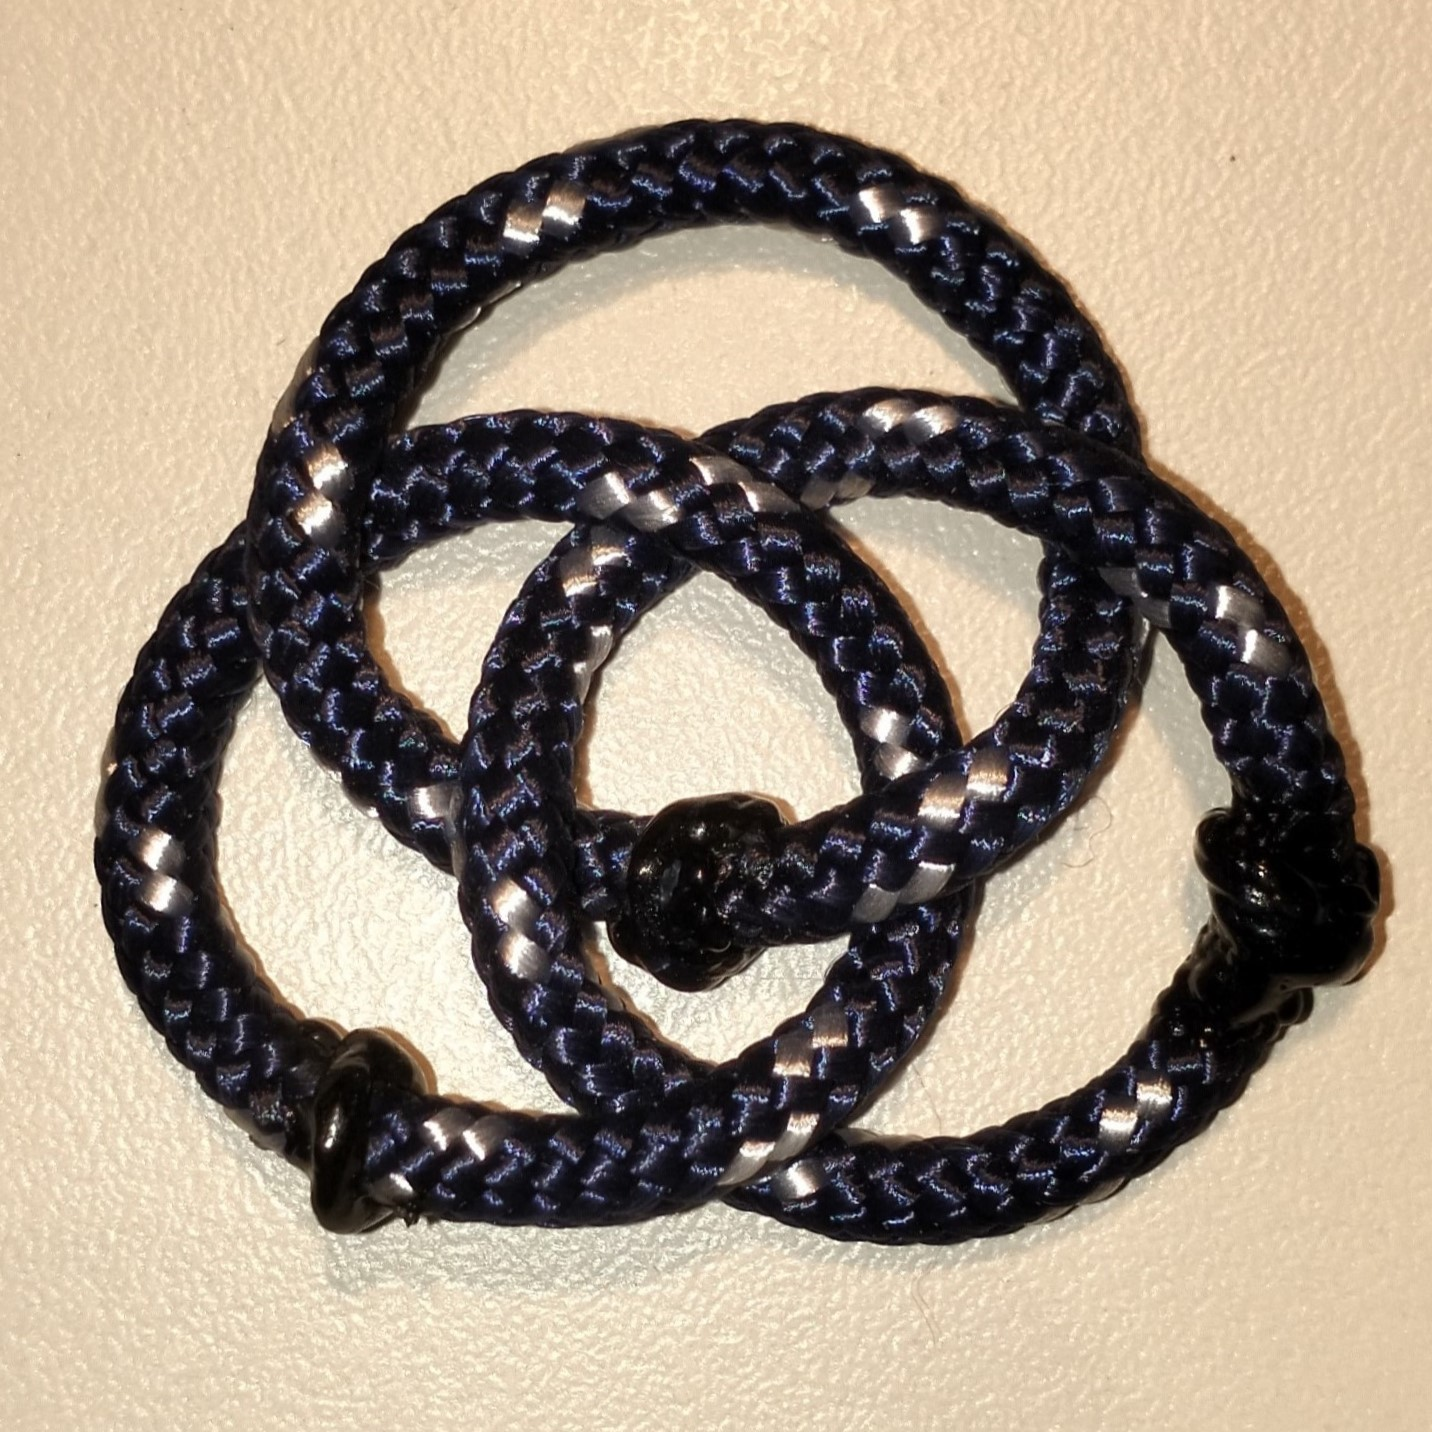
\includegraphics[width=0.45\linewidth]{img/anell borromeu.jpg}
	\caption{A l'esquerra el nus $7_1$ (més endavant explicarem el perquè del nom). A la dreta un 3-link conegut amb el nom d'anell Borromeu. 
	}\label{fig:exemplesdenusosenmatematiques}
\end{figure}

\begin{definition}
	Diem que un nus està \underline{desnuat} o que és el nus trivial, notacionalment $\ovoid$ si no presenta cap creuament en els segments de corda que el formen.
\end{definition}

\subsection{Equivalència entre nusos}\label{Equivalència entre nusos}

Expliquem ara què entem quan diem que dos nusos son el mateix.

\begin{definition}\label{def: Definició d'isotopia ambient}
	Diem que dos links $L$ i $L'$ a $S^3$ son equivalents si existeix una isotopia ambient entre ells.
\end{definition}
És a dir, si existeix una família d'homeomorfismes $h_t:S^3\rightarrow S^3$ per $t\in[0, 1]$ tal que $h_0=1$, $h_1=h$ i $(x, t)\mapsto(h_{t}x, t)$ és un homeomorfisme lineal a trossos de $S^3\times[0, 1]$ a $S^3$, llavors direm que $L$ i $L'$ son links equivalents. L'equivalència entre nusos és la mateixa que en la Definició \ref{def: Definició d'isotopia ambient} tenint present que en aquest cas només tenim una component. Observem que la distorsió no és del mateix link sinó de l'espai "ambient" $S^3$ en sí mateix. Definir nus equivalent d'aquesta manera evita que els creuaments que formen el nus o link puguin fer-se cada vegada més petits fins a desapareixer. D'aquesta manera, és possible moure tot $S^3$ de forma contïnua utilitzant $h_t$ per passar de $L$ a $L'$.

\subsection{Representació d'un nus en matemàtiques}\label{sec:Representació de nus}
Tenint present la definició de nus a partir d'ara en sentit matemàtic donada a la Definició \ref{def: Definició de nus}, un pot veure la dificultat d'estudiar aquest tipus d'objectes tres dimensionals en un llibre de text o bé en una pissarra. És per això, que per tal d'estudiar-los sovint es representen els nusos mitjançant el seu \textit{diagrama de nus}.\\

Considerant la projecció paral·lela (o axonomètrica) sobre l'eix $z$ en el pla $\mathbb{R}^2$ d'un nus qualsevol $K$, obtindrem una figura com en l'exemple \ref{fig:projecció d'un nus sobre R2}.\\

\begin{figure}
	\centering
		\resizebox{7.5cm}{!}{
			
			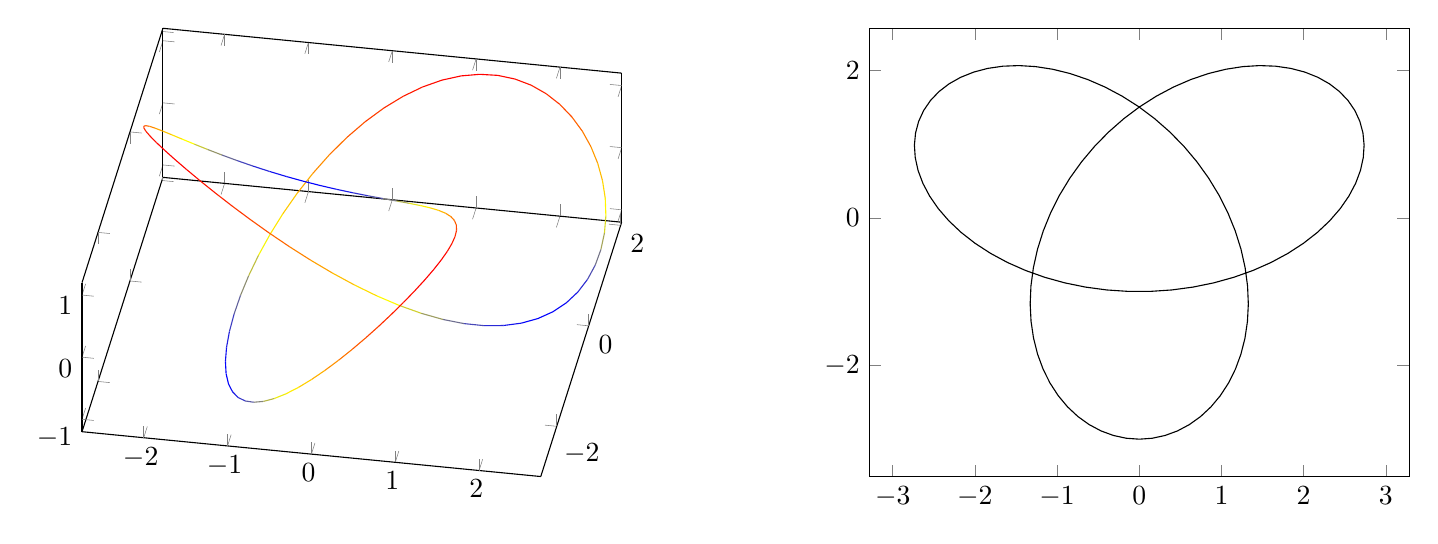
\begin{tikzpicture}
				
				\begin{scope}
					\begin{axis}
						\addplot [domain=-pi:pi,samples=120]({sin(deg(x))+2*sin(2*deg(x))},{cos(deg(x))-2*cos(2*deg(x))}); 
					\end{axis}
				\end{scope}
				
				\begin{scope}[xshift=-10cm]
					\begin{axis}
						[
						view={10}{60},
						]
						\addplot3[
						domain=-pi:pi,
						samples = 120,
						samples y=0,
						mesh
						]
						({sin(deg(x))+2*sin(2*deg(x))},
						{cos(deg(x))-2*cos(2*deg(x))},
						{-1*sin(3*deg(x))});
					\end{axis}
				\end{scope}
				
			\end{tikzpicture}
			
		}
	\caption{A l'esquerra el nus $3_1$ també conegut com Trefoil amb parametrització $(\sin t+2\sin 2t, \cos t-2\cos 2t,-\sin 3t)$. A la dreta, la seva projecció paral·lela sobre l'eix $z$.}\label{fig:projecció d'un nus sobre R2}
\end{figure}

Considerant aquesta projecció però, un perd informació sobre el propi nus, ja que cal saber quin segment de corda va per sobre i quin per sota alhora de creuar-se. Per tal de no perdre aquesta informació, el segment que passa per sota se'l dibuixa de forma discontínua mentre aquest passa sota el segment de corda que el creua.\\

\noindent
D'aquesta manera, la projecció del nus $3_1$ de la Figura \ref{fig:projecció d'un nus sobre R2} quedaria de la següent manera:

\begin{figure}[H]
	\resizebox{6.5cm}{!}{
		\begin{tikzpicture}[line width=0.5mm]
			\begin{scope}[rotate=270]
				\begin{knot}[
					consider self intersections=true,
					%  draft mode=crossings,
					flip crossing=2,
					only when rendering/.style={
						%    show curve controls
					}
					]
					\strand (0,2) .. controls +(2.2,0) and +(120:-2.2) .. (210:2) .. controls +(120:2.2) and +(60:2.2) .. (-30:2) .. controls +(60:-2.2) and +(-2.2,0) .. (0,2);
				\end{knot}
			\end{scope}
			
			\begin{scope}[xshift=-5cm, rotate=270]
				\begin{knot}[
					consider self intersections=false,
					%  draft mode=crossings,
					flip crossing=2,
					only when rendering/.style={
						%    show curve controls
					}
					]
					\strand (0,2) .. controls +(2.2,0) and +(120:-2.2) .. (210:2) .. controls +(120:2.2) and +(60:2.2) .. (-30:2) .. controls +(60:-2.2) and +(-2.2,0) .. (0,2);
				\end{knot}
			\end{scope}
		\end{tikzpicture}
	}
\end{figure}

Així doncs, considerant la projecció paral·lela sobre l'eix $z$ d'un nus $K$ qualsevol i disposant de la informació sobre els creuaments obtenim el que anomenarem \textit{diagrama de nus}, notacionalment $diag(K)$. Moltes vegades, en la literatura es fa un abús de llenguatge i notació, anomenant nus al que nosaltres anomenem diagrama de nus i fent servir $K$ i $diag(K)$ indistintament. D'aquí a no massa veurem que de fet, estudiar-ne les propietats d'un és equivalent a estudiar les de l'altre.\\
	% !TEX root = thesis.tex

\section{Els moviments de Reidemeister}\label{sec:Reidermeister}
Una primera aproximació per tal de distingir si dos nusos son diferent és veure quan son iguals. Aquesta és la inspiració darrera de la següent secció que tractarà sobre els moviments de Reidemeister i el Teorema central de la Teoria de Nusos.

\subsection{Moviments de Reidemeister}\label{subsec:Moviments de Reidemeister}
Motivats per la Secció \ref{Equivalència entre nusos}, un podria veure sense massa dificultat que cadascun dels moviments de la Figura \ref{fig:Moviments de Reidemeister} resulta en un diagrama de nus equivalent a l'original.\\

\begin{figure}[h]
	\centering
	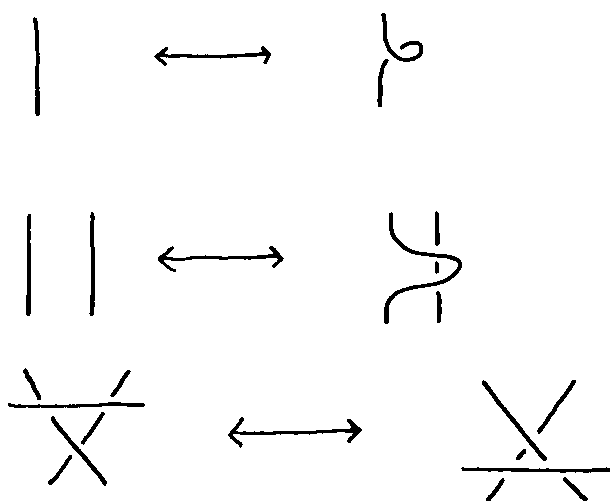
\includegraphics[width=0.9\linewidth]{img/MovimentsdeReidemeister.png}
	\caption{De dalt a baix: Moviment de Tipus I, Tipus II i Tipus III  [\cite{SobreelsmovdeReide}]. Cal pensar que els segments lliures de corda s'uneixen a través d'un nus $K$.}\label{fig:Moviments de Reidemeister}
\end{figure}

A aquests tres tipus de moviments se'ls anomena moviments de Reidemeister. Al primer de tots se'l diu de Tipus I o \textit{twist} en anglès, al segon de Tipus II o \textit{poke} i al tercer de Tipus III o \textit{slide}.\\

\noindent
\textbf{Moviment de Tipus I o \textit{twist}:} També anomenat \textbf{RI} per abreujar notació, aquest tipus de moviment consisteix en "pessigar" la corda i amb el tros obtingut donar-li la volta (d'aquí el nom en anglès) fent un bucle com en el de la Figura \ref{fig:Moviments de Reidemeister}.\\

\noindent
\textbf{Moviment de Tipus II o \textit{poke}:} També anomenat \textbf{RII}. Aquest tipus de moviment consisteix en fer passar una de les dues cordes per sobre de l'altra. En anglès, la paraula \textit{poke} significa fer passar forçosament alguna cosa en una certa direcció i doncs en aquest cas es podria pensar que una de les dues cordes s'ha fet passar per sobre de l'altra.\\

\noindent
\textbf{Moviment de Tipus III o \textit{slide}:} També anomenat \textbf{RIII}. Aquest tipus de moviment consisteix en, com el nom en anglès indica, fer lliscar una de les tres cordes d'una banda a l'altra de la intersecció entre les dues cordes restants. En la Figura \ref{fig:Moviments de Reidemeister} podem veure com el segment de corda horitzontal llisca de dalt a baix del creuament entre les altres dues cordes.\\

Continuant amb el que hem vist, no és massa difícil veure que aplicant una seqüència finita de moviments RI, RII o RIII a un diagrama de nus qualsevol, el nus obtingut és equivalent a l'original.

\subsection{El Teorema central de la Teoria de Nusos}\label{sec:teoremacentraldelateoria}

L'any 1930, Kurt Reidemeister demostrà que l'implicació contrària també és certa, és a dir que si dos diagrames de nusos qualssevol son equivalents, aleshores sempre podem trobar una seqüència finita de moviments de Reidemeister de manera que podem transformar un diagrama de nus en l'altre. Aquest resultat va donar lloc al teorema central de la teoria.

\begin{theorem}\label{teo:teoremadeReidemeister}
   $diag(K)$ i $diag(K')$ son equivalents si i només si, existeix una seqüència finita de moviments RI, RII o RIII que passa d'un a l'altre.
\end{theorem}

Una demostració del teorema original es pot trobar a (Knot Knotes Justin Roberts, pàgina 18 Teorema 2.3.1) \cite{knotentheorie}, \textbf{però en essència aquesta demostració fa ús del fet que la manera en que un pot generar nusos equivalents a l'original és a través d'afegir triangles als costats d'un nus poligonal.}\\

\begin{figure}[H]
	\centering
	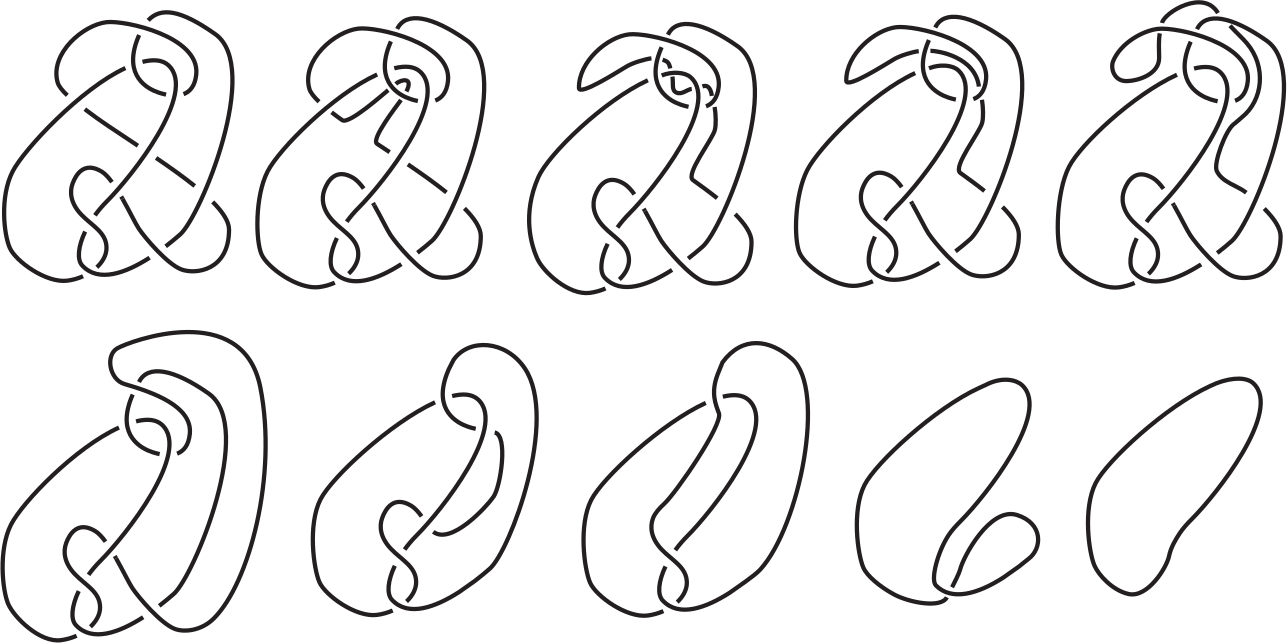
\includegraphics[width=0.9\linewidth]{img/culprit-knot.png}
	\caption{Com es pot observar en l'exemple, el nus de Culprit és equivalent al nus zero o \textit{unknot} en anglès. Mitjançant la seqüència de moviments següent podem passar de l'un a l'altra. D'esquerra a dreta i de dalt a baix: RII, RIII+RIII, RII, RIII, RI+RII, RII, RII, RII, RI, [\cite{culpritknot}].}\label{fig:culpritknot}
\end{figure}

El Teorema \ref{teo:teoremadeReidemeister} doncs, posa en evidència el fet que parlar d'equivalència entre nusos o d'equivalència entre diagrames de nusos és el mateix, doncs aquests estan en correspondència a través de la Secció \ref{sec:Representació de nus}.\\

D'aquesta manera i fent referència al mencionat anteriorment, a partir d'ara farem un abús de llenguatge i notació dient nus $K$ indistintament sense posar importància al fet de si ens referim al nus o al seu diagrama.
	% !TEX root = thesis.tex

\section{Propietats sobre nusos}\label{sec:Propietats_sobre_nusos}

En aquesta Secció posarem de manifest diferents propietats d'un nus que més endavant tindran importància en la seva classificació.

\begin{definition}\label{def:ordre}
	Anomenem \underline{ordre} de $K$, $O(K)$ al mínim nombre de creuament que aquest pot arribar a presentar donat un diagrama qualsevol.
\end{definition}

La Figura \ref{fig:culpritknot} demostra que l'ordre del nus Culprit és zero ja que aquest sempre és un nombre positiu. Tampoc és molt difícil veure que donat un nus $K$ qualsevol a aquest se li pot afegir creuaments mitjançant moviments RI, no obstant $O(K)$ es manté contant.

\begin{definition}\label{def:nusemmirallat}
	Diem que un nus és l'\underline{emmirallat} $\overline{K}$ d'un altre nus $K$ si aquest primer s'obté a partir de l'original canviant tots els creuaments de sobrepassos a sotapassos i a la inversa.
\end{definition}

La Figura \ref{fig:nus emmirallat} mostra un exemple d'un nus emmirallat.\\

\begin{figure}
	\resizebox{6.5cm}{!}{
		\begin{tikzpicture}[line width=0.5mm, use Hobby shortcut]
			\begin{scope}
				\begin{knot}[
					consider self intersections=true,
					%  draft mode=crossings,
					ignore endpoint intersections=false,
					flip crossing/.list={1,5,6},
					only when rendering/.style={
						%    show curve endpoints
					}
					]
					\strand ([closed]0,0) .. (1.5,1) .. (.5,2) .. (-.5,1) .. (.5,0) .. (0,-.5) .. (-.5,0) .. (.5,1) .. (-.5,2) .. (-1.5,1) .. (0,0);
				\end{knot}
				\path (0,-.7);
			\end{scope}
			
			\begin{scope}[xshift=-5cm]
				\begin{knot}[
					consider self intersections=true,
					%  draft mode=crossings,
					ignore endpoint intersections=false,
					flip crossing/.list={3,4},
					only when rendering/.style={
						%    show curve endpoints
					}
					]
					\strand ([closed]0,0) .. (1.5,1) .. (.5,2) .. (-.5,1) .. (.5,0) .. (0,-.5) .. (-.5,0) .. (.5,1) .. (-.5,2) .. (-1.5,1) .. (0,0);
				\end{knot}
				\path (0,-.7);
			\end{scope}
		\end{tikzpicture}
	}
	\caption{A l'esquerra el nus $4_1$ o Figure Eight en Anglès. A la dreta, el seu nus emmirallat.}\label{fig:nus emmirallat}
\end{figure}

D'aquesta manera, si un nus $K$ és equivalent a $\overline{K}$, llavors diem que és \textit{amfiquiral}, sinó diem que és \textit{quiral}. El nus $4_1$ de la Figura \ref{fig:nus emmirallat} és un exemple de nus amfiquiral, però no sempre és veritat que un nus $K$ sigui equivalent a $\overline{K}$ com veurem més endavant.

\begin{definition}\label{def:nusinvers}
	Diem que un nus és l'\underline{invers} $rK$ d'un altre nus $K$ si aquest primer s'obté a partir de l'original canviant-ne l'orientació.
\end{definition}

És clar que un nus pot ser orientat de dues maneres diferents, escollir una d'aquestes orientacions és informació extra sobre el nus que pot o no ser donada. De manera similar a la Definició \ref{def:nusemmirallat}, no sempre un nus és equivalent al  seu invers.

\begin{figure}
	\centering
	\includegraphics[width=0.6\linewidth]{img/orientació.png}
	\caption{Les dues úniques orientacions del nus trivial. És evident que aquests dos diagrames son equivalents.}\label{fig:nusorientat}
\end{figure}

\begin{definition}
	Diem que un nus $K$ és \underline{primer} si no és el nus trivial i si $K=K_1+K_2$ implica que $K_1$ o $K_2$ és el nus trivial.
\end{definition}

En aquest cas, el símbol $+$ fa referència a l'operació suma. Donats dos nusos orientats $K$ i $K'$, aquests poden ser sumats posant-los un al costat de l'altre i unint-los de manera que es preservi l'orientació. Aquesta operació està ben definida sota equivalència. A més, és commutativa, associativa i té element neutre. Més endavant estudiarem aquesta operació en detall AAAAAAAAAAAAAAAAAAAAAAAA.\\

\begin{figure}
	\centering
	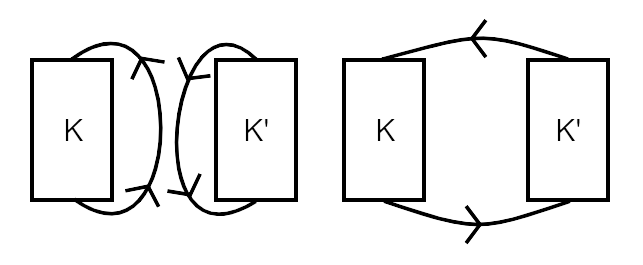
\includegraphics[width=0.9\linewidth]{img/nussuma.png}
	\caption{Suma de dos nusos qualssevol.}\label{fig:nussuma}
\end{figure}

La Figura \ref{fig:knotable} és una taula que conté tots els nusos primers de fins a 9 creuaments. Cadascun rep un nom conformat per un parell de nombres; el primer de tots correspon al seu ordre i el segon és un subíndex històricament assignat a aquell nus en concret. Les primeres tabulacions que es coneixen van fer-se per Tait l'any 1860 mentre aquest estudiava l'àtom. Aquesta taula negligeix el fet que possiblement un mateix nus $K$ sigui diferent a $\overline{K}$, $rK$ o $\overline{rK}$. D'aquesta manera, cada nus de la taula correspon a un, dos o quatre nusos de $S^3$ mitjançant les operacions definides a \ref{def:nusemmirallat} i \ref{def:nusinvers}.

\begin{figure}
	\centering
	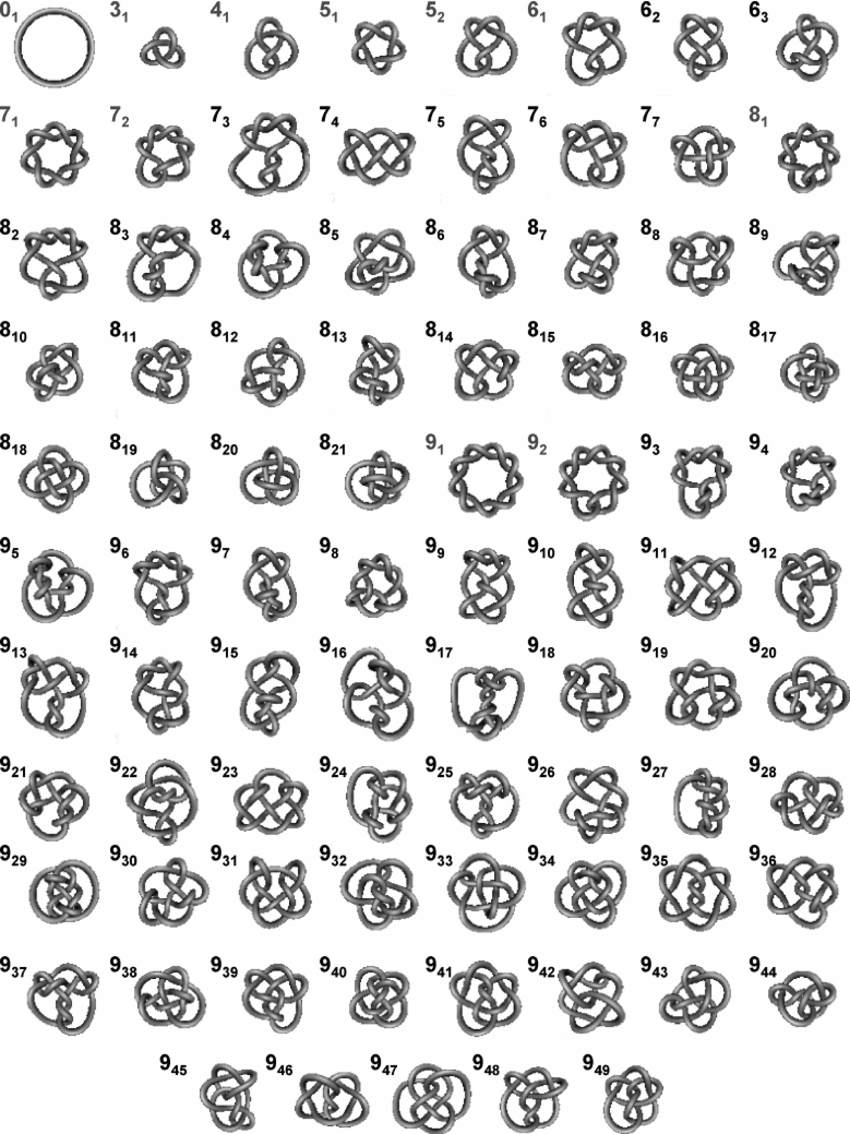
\includegraphics[width=0.9\linewidth]{img/knottable.png}
	\caption{Taula de nusos fins a ordre 9.}\label{fig:knotable}
\end{figure}

\begin{definition}\label{def:nusalternat}
	Diem que $K$ és un nus \underline{alternat} si a mesura que anem recorrent el nus, els creuaments alternen de sobrepassos a sotapassos.
\end{definition}

El nus $4_1$ n'és un exemple. De fet, cal anar fins a $8_{19}$ per trobar el primer nus no alternat i doncs això és una conseqüència del baix ordre dels nusos. Es pot veure que donat un ordre qualsevol, sempre existeix com a mínim un nus alternat. Ara bé, aquests disminueixen exponencialment a mesura que incrementem l'ordre del nus. Aquesta classe de nusos tenen bones propietats.
	\input{Alguns_invariants_algebràics.tex}
	% !TEX root = thesis.tex

\section{El polinomi de Jones}\label{sec:El polinomi de Jones}

El descobriment del \textit{polinomi de Jones} per part de Vaughan Jones l'any 1984 [\cite{jonesoriginal}] dona una manera d'associar a cada nus o link un polinomi de Laurent amb coeficients enters. Aquesta correspondència es fa mitjançant un diagrama de link qualsevol. La teoria de Jones es fonamenta en el fet que si fem un moviment RI, RII o RIII al diagrama del link, aquest polinomi no canvia i doncs és un invariant sota moviments de Reidemeister. El polinomi per un link és doncs independentment del diagrama d'aquest. De manera que si podem veure que dos diagrames de links no tenen el mateix polinomi, llavors segur que aquests son diferents.\\

La manera més simple per definir-lo és mitjançant un altre tipus de polinomi; el \textit{polinomi de Kauffman} descobert per Louis Kauffman.\\

\begin{definition}
	El \underline{polinomi de Kauffman} de $L$, $\langle L\rangle$ és un polinomi de Laurent amb coeficients enters i indeterminada $A$ que podem associar a tot diagrama d'un link a $S^2$ de la següent manera:
	\begin{enumerate}
		\item\label{item:i} $\left\langle\KPA\right\rangle=1$
		\item\label{item:ii} $\left\langle L \cup \KPA\right\rangle=(-A^{-2}-A^{2})\langle L\rangle$
		\item\label{item:iii} $\left\langle\KPB\right\rangle=
		A\left\langle\KPC\right\rangle + A^{-1} \left\langle \KPD \right\rangle$
	\end{enumerate}
\end{definition}

En aquesta definició, $$\KPA$$ és el diagrama del nus zero i $$L \cup \KPA$$ és un diagrama de $L$ juntament amb una corba tancada extra que no conté cap creuament ni amb ella mateixa ni amb $L$. A \textit{\ref{item:iii}} la fórmula relaciona tres diagrames que son el mateix excepte al voltant d'un creuament on es diferencien pels moviments locals indicats. A partir d'aquesta definició és fàcil veure les següents propietats.

\begin{itemize}
	\item $\left\langle\KPA\stackrel{c}{\dots}\KPA\right\rangle=(-A^{-2}-A^{2})^{c-1}$
	\item $\left\langle L\right\rangle=\left\langle rL\right\rangle$
\end{itemize}

La Figura \ref{fig:calculpolinomidekauffman} mostra de forma iterativa el càlcul d'aquest polinomi. Així doncs trobem que $$\left\langle 3_1\right\rangle=A^{-7}-A^{-3}-A^{5}$$ Un exercici similar demostra que $$\left\langle \overline{3_1}\right\rangle=A^{7}-A^{3}-A^{-5}$$

Investiguem ara el comportament del polinomi respecte els moviments de Reidemeister.

\begin{lemma}\label{lem:RI}
	Si a $K$ hi apliquem un moviment RI el seu polinomi de Kauffman canvia de la següent manera $$\left\langle FALTAAAA\right\rangle$$
\end{lemma}

\begin{proof}
	Utilitzant \textit{\ref{item:iii}} i \textit{\ref{item:ii}} en aquest mateix ordre.
\end{proof}

Notem a més que si a \textit{\ref{item:iii}} fessim un moviment local canviant-lo a $$\KPI$$ llavors el polinomi de Kauffman corresponent seria el mateix que l'original intercanviant $A$ per $A^{-1}$. Això significa que si $\overline{K}$ és el nus emmirallat de $K$, llavors $\left\langle\overline{K}\right\rangle=\overline{\left\langle K\right\rangle}$, on $\overline{\left\langle K\right\rangle}$ denota el canvi esmentat anteriorment. Així, observant la Proposició \ref{lem:RI} deduïm que $$FALTA$$ En l'exemple del càlcul del polinomi de Kauffman de $3_1$ anterior també es dona aquest cas.

\begin{figure}
	\centering
	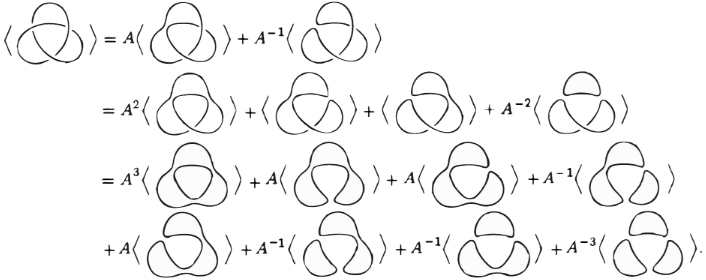
\includegraphics[width=0.9\linewidth]{img/polinomidekauffman.png}
	\caption{Exemple del polinomi de Kauffman de $3_1$.}\label{fig:calculpolinomidekauffman}
\end{figure}

\begin{lemma}\label{lem:RIIiRIII}
	El polinomi de Kauffman és invariant per moviments RII i RIII
\end{lemma}

\begin{proof}
	Per RII cal aplicar \textit{\ref{item:iii}} dues vegades seguides sabent que $\left\langle\overline{K}\right\rangle=\overline{\left\langle K\right\rangle}$ i aplicar-ho en un dels dos creuaments. Per RIII igual.
\end{proof}

\begin{definition}\label{def:torçament}
	Definim el \underline{torçament} $w(L)$ del diagrama d'un link orientat qualsevol com la suma dels signes dels seus creuaments, on cada un d'aquests pren el valor $+1$ o $-1$ com s'indica a la Figura \ref{fig:signe}
\end{definition}

\begin{figure}
	\centering
	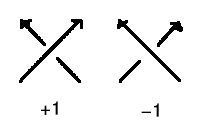
\includegraphics[width=0.9\linewidth]{img/signe.jpg}
	\caption{Signe d'un creuament per la regla de la ma dreta.}\label{fig:signe}
\end{figure}

Notem que la Definició \ref{def:torçament} utilitza la orientació del link. Notem també que aquest és invariant sota moviments RII i RIII i aquest canvia per $+1$ o $-1$ sota moviments RI. La Figura \ref{fig:calculdelsigne} mostra dos exemples sobre el càlcul del torçament d'un nus.\\

\begin{figure}
	\centering
	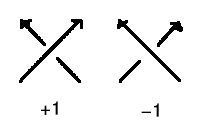
\includegraphics[width=0.9\linewidth]{img/signe.jpg}
	\caption{A l'esquerra el nus $5_1$ que té torçament -5, a la dreta $r5_1$ que té torçament -5.}\label{fig:calculdelsigne}
\end{figure}

El troçament d'un link orientat juntament amb el polinomi de Kauffman d'un diagrama de link sense tenir en compte l'orientació son tots dos invariants sota moviments RII i RIII a més, aquests es comporten d'una manera previsible sota moviments RI. Això duu al següent resultat:

\begin{theorem}
	Sigui $diag(L)$ un diagrama d'un link orientat $L$. Llavors, $$(-A)^{-3w(L)}\left\langle L\right\rangle$$ és un invariant del link orientat $L$.
\end{theorem}

\begin{proof}
	Conseqüència directa del Lema \ref{lem:RIIiRIII}, el Lema \ref{lem:RI} i l'observació sobre el torçament sota moviments $RI$ anterior.
\end{proof}
	% !TEX root = thesis.tex

\section{Aplicacions}\label{sec:Aplicacions}
	\clearpage
	
	\bibliographystyle{plainnat}
	\bibliography{sample}
\end{document}